\chapter{RTL blocks}
\label{chapter:rtl}

This section introduces the RTL modules or ``RTL blocks'' which were developed and characterized for this work. The characterization \textit{process} will be discussed in Section~\ref{chapter:framework}.

\section{Scalar RTL blocks}

This work provides characterized RTL blocks for:

\begin{itemize}
    \item Arithmetic

    \begin{itemize}
        \item Adder
        \item Subtractor
        \item Multiplier
    \end{itemize}
    
    \item Comparison

    \begin{itemize}
        \item Equality comparator
    \end{itemize}
\end{itemize}

These straightforward circuits are useful as building blocks for other RTL designs, and the characterization metrics for these circuits are useful building-blocks for modeling.

These components are all parameterized by \textbf{operand bitwidth}. All of these components are scalar, processing one operand (or pair of operands) per cycle and producing one output.

\section{Vectorized RTL blocks}

All ``vectorized' RTL blocks consume vector inputs and yield vector outputs. Depending on implementation, the degree of input and output vectorization may be determined by separate parameters (as is the case for the ``skip-ahead'' intersection unit) or by a single parameter (as is the case for the two-fingered merge-based intersection unit.)

Here, ``vectorization'' is used to mean that (1) the input and output data structures of the RTL block are vectors, and (2) the processing throughput is such that all vector operands are consumed within a cycle, and each vector output is produced in its entirety within a cycle.

Notably, an RTL block being ``vectorized'' is decoupled from the degree of parallelism of the underlying combinational logic. The vectorized ripple prefix-sum, for example, uses a linear-depth design based on chained adders in order to process a vector of inputs within a cycle (provided that the critical path latency complies with the clock latency), while the vectorized parallel Kogge-Stone\cite{koggestone} prefix-sum uses a log-depth tree design that trades off higher area for sub-linear critical path length scaling.

\subsection{Vector pipelining and combinational unrolling}

Some RTL blocks such as prefix-sum naturally consume a vector and output a vector.

However, other blocks such as coordinate-payload intersection units and priority encoder, consume a vector and output a single value. A method is needed to increase the throughput of these components in cases where one-result-per-cycle is insufficient.

Previous works such as ExTensor\cite{extensor} rely on vector pipelining in order to increase the throughput of intersection units. Although the structure of the vector pipeline is not laid out explicitly, one can imagine how such a vector pipeline might be implemented: first implement a single stage which is equivalent to one ``step'' of the intersection process; the stage should accept a state vector representing the progress toward completing the intersection, and should output (1) at most one and at least zero matches which were discovered by the stage, and (2) an updated state vector. Second, cascade multiple stages, such that the output of the cascade is an updated state vector reflecting \textit{multiple} stages of the intersection process, as well as potentially multiple intersection matches which were discovered.

In the context of this work, two ways of creating staged RTL are relevant:

\begin{itemize}
    \item \textbf{Vector pipelining.} Multiple stages are daisy-chained but separated by registers; each pipeline stage is a single intersection stage. \textbf{Propagation delay requirement:} the propagation delay of a single stage must be less than the clock period, minus margin.
    \item \textbf{Combinational unrolling.} Multiple stages are daisy-chained and \textbf{combinationally-connected without pipeline registers}; the whole multi-stage intersection unit constitutes a single pipeline stage. \textbf{Propagation delay requirement:} the propagation delay \textbf{of the whole multi-stage intersection unit} must be less than the clock period, minus margin.
\end{itemize}

The benefit of vector pipelining is the more lenient propagation delay requirement; empirically, a more lenient propagation delay requirement appears to also results in lower power consumption and area per-stage after gate-level synthesis.

The benefits of combinational unrolling are that (1) the energy and area overhead of pipelining registers avoided, and (2) there is no need orchestrate control signals between pipeline stages. However, besides the propagation delay, an additional drawbacks is that combinational unrolling can have non-linear overheads resulting from i.e. the logic which compacts the matches found by multiple intersection stages into a single vector.

In this work, each RTL block is parameterized, and then characterized over a range of \textbf{combinational unrolling} depths, starting at 1. In future work it could be valuable to explore vector pipelining as well.

\subsubsection{Chaining}

As described above, vector pipelining and combinational unrolling are implemented here in such a way that each stage is identical, and an updated state vector is passed from stage to stage.

What if an operation such as intersection is not completed in a single pass through the vector pipeline/combinational intersection unit? There is nothing to prevent \textit{chaining}, i.e. collecting the state vector at the output of the vector pipeline/combinational intersection unit, and feeding it back to the input. 

With chaining, the size of the vector pipeline/combinational unrolling does not affect the feasibility of a computation, only its runtime.

\subsection{Prefix-sum units}

Prefix sum does not require vector pipelining or combinational unrolling.

\textbf{Vectorized prefix sum parameters:}

\begin{itemize}
    \item Input vector length
    \item Word bits
\end{itemize}

\textbf{RTL implementations for the following prefix sum designs (all sharing the above parameter list) are provided:}

\begin{itemize}
    \item \textbf{Ripple prefix-sum:} linear-depth prefix-sum implementation based on chained adders.
    \item \textbf{Parallel Kogge-Stone\cite{koggestone} prefix-sum:} log-depth prefix-sum implementation based on adder trees.
\end{itemize}

\subsubsection{Kogge-Stone prefix-sum}

\begin{figure}[H]
    \centering
    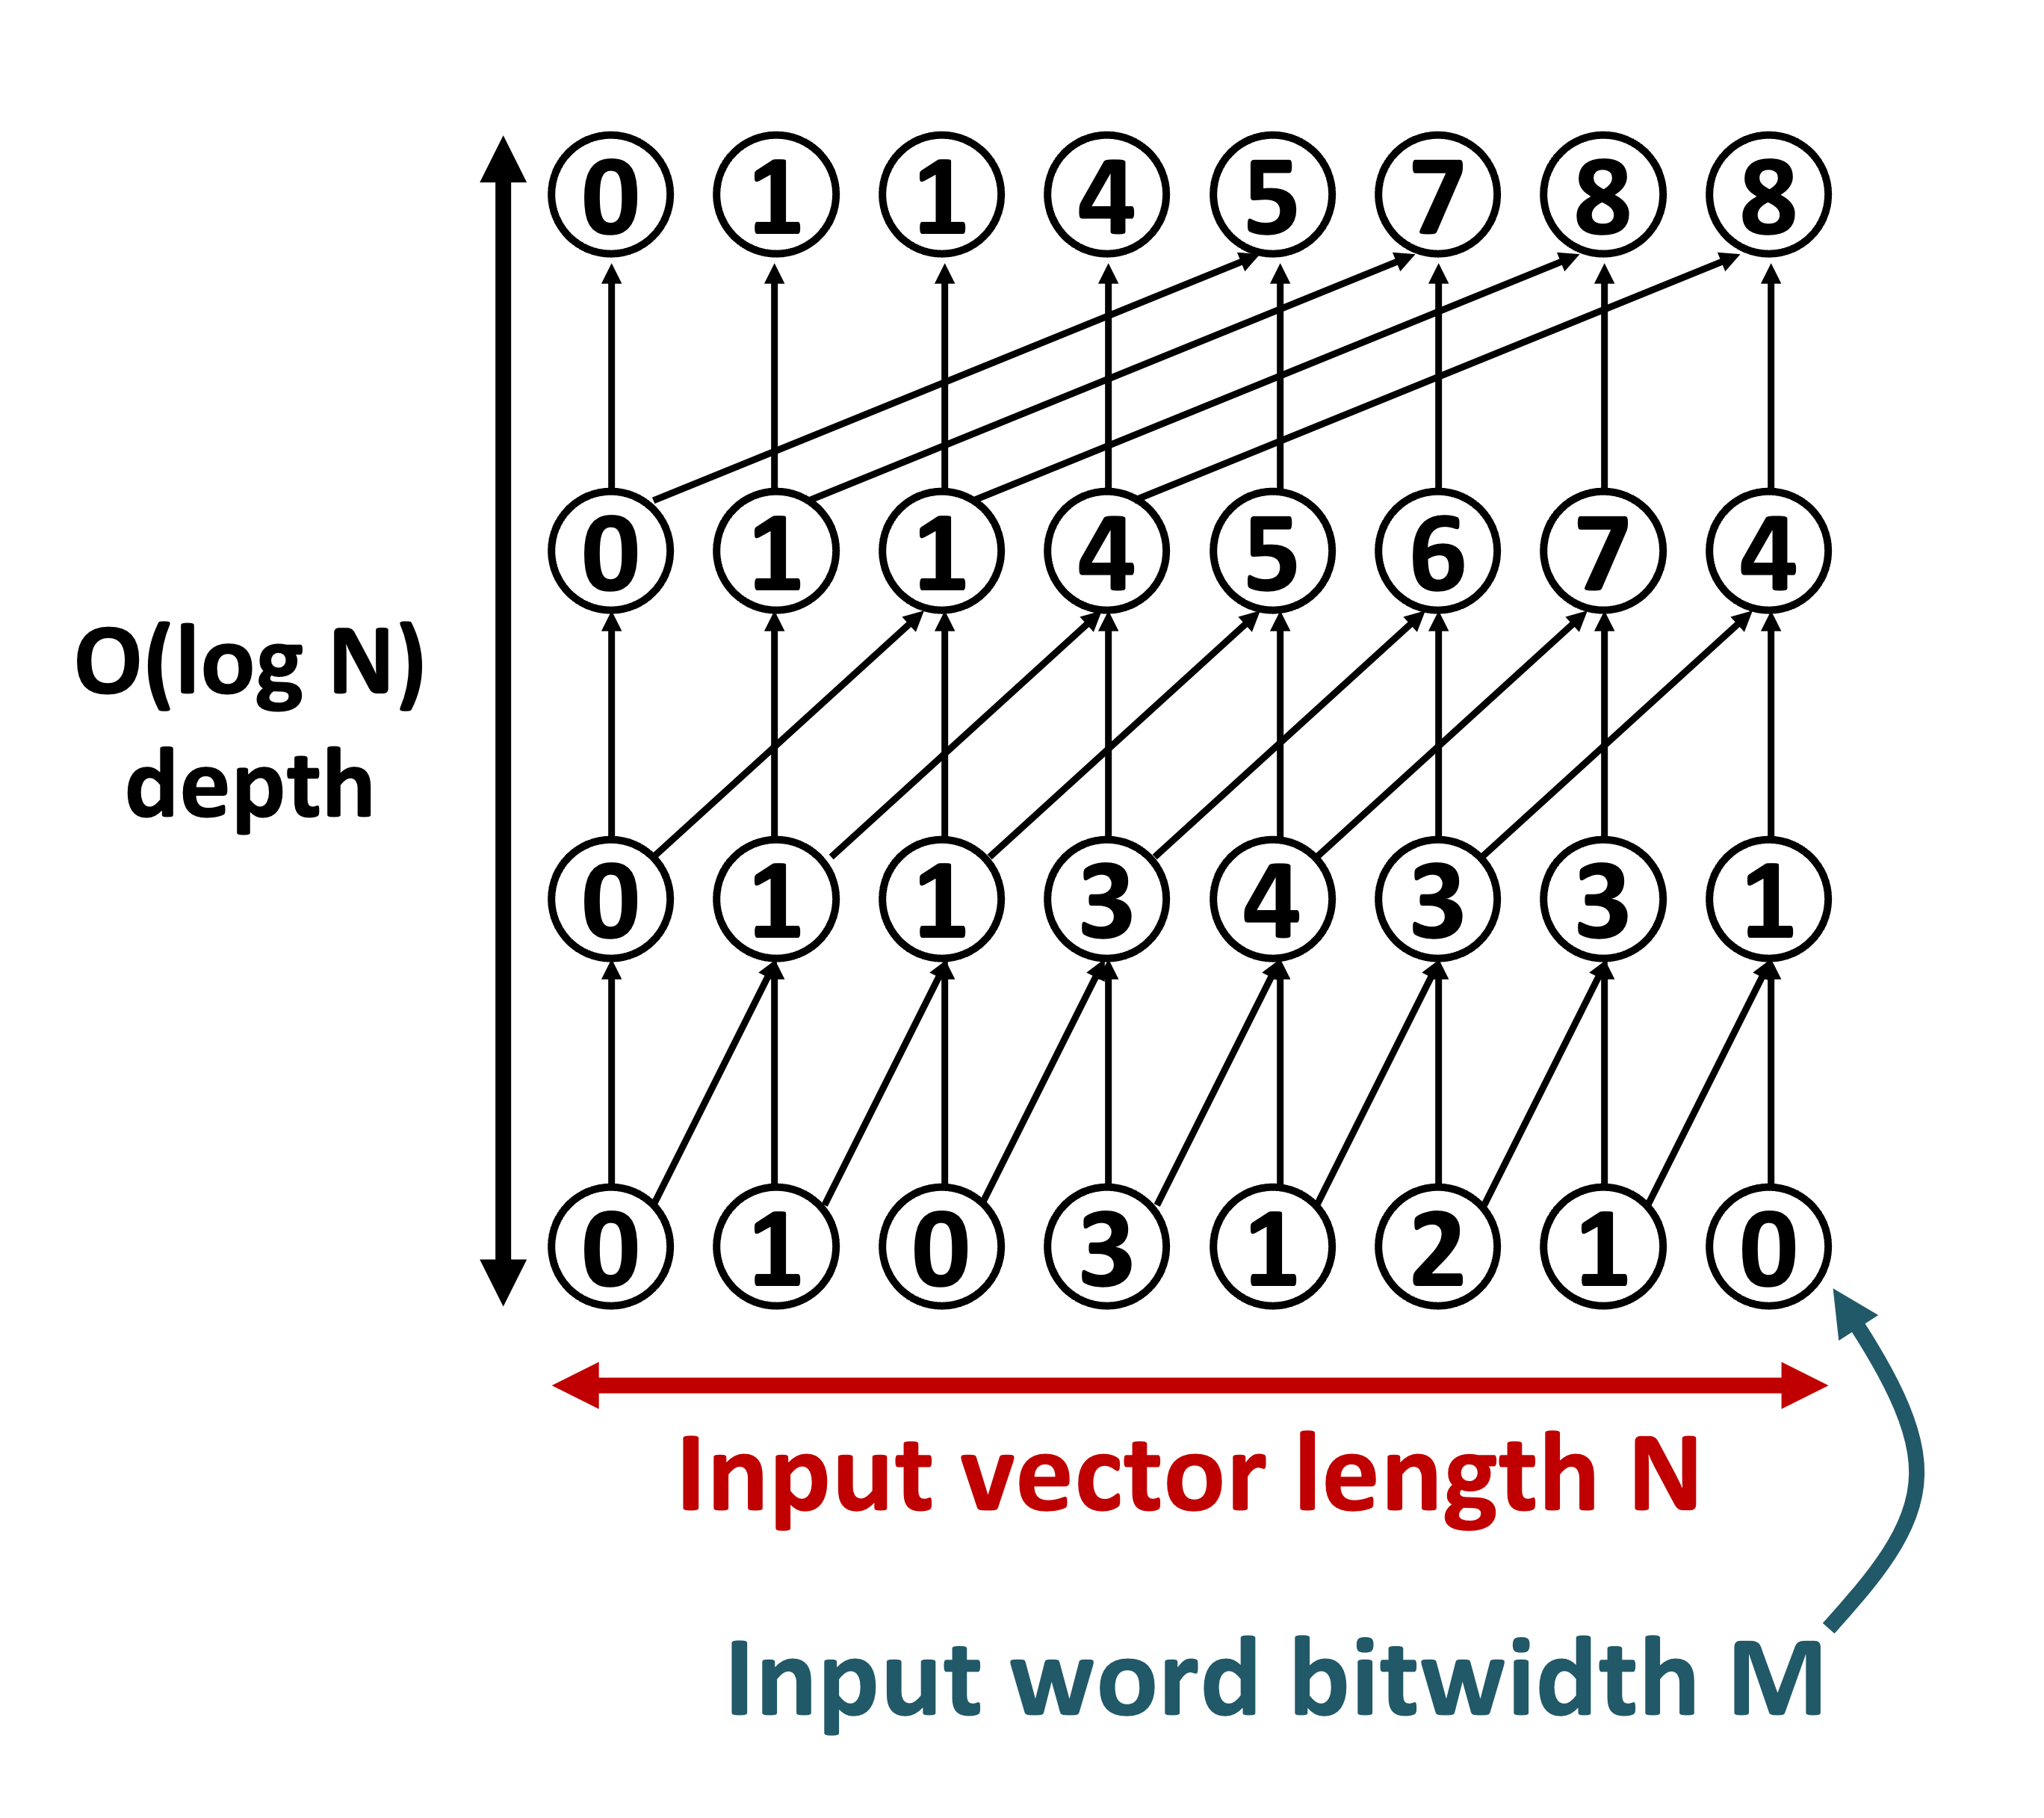
\includegraphics[width=0.95\textwidth]{figures/kogge_stone_prefix_sum.png}
    \caption{The Kogge-Stone\cite{koggestone} prefix-sum RTL block implements a log-depth vectorized prefix-sum with a 1-stage vector pipeline (registered I/O.) It is parameterized by \textbf{input word bitwidth} and \textbf{degree of vectorization.}}
    \label{fig:kogge_stone_prefix_sum}
\end{figure}

Figure~\ref{fig:kogge_stone_prefix_sum} summarizes Kogge-Stone prefix-sum.

\subsubsection{Ripple prefix-sum}


\begin{figure}[H]
    \centering
    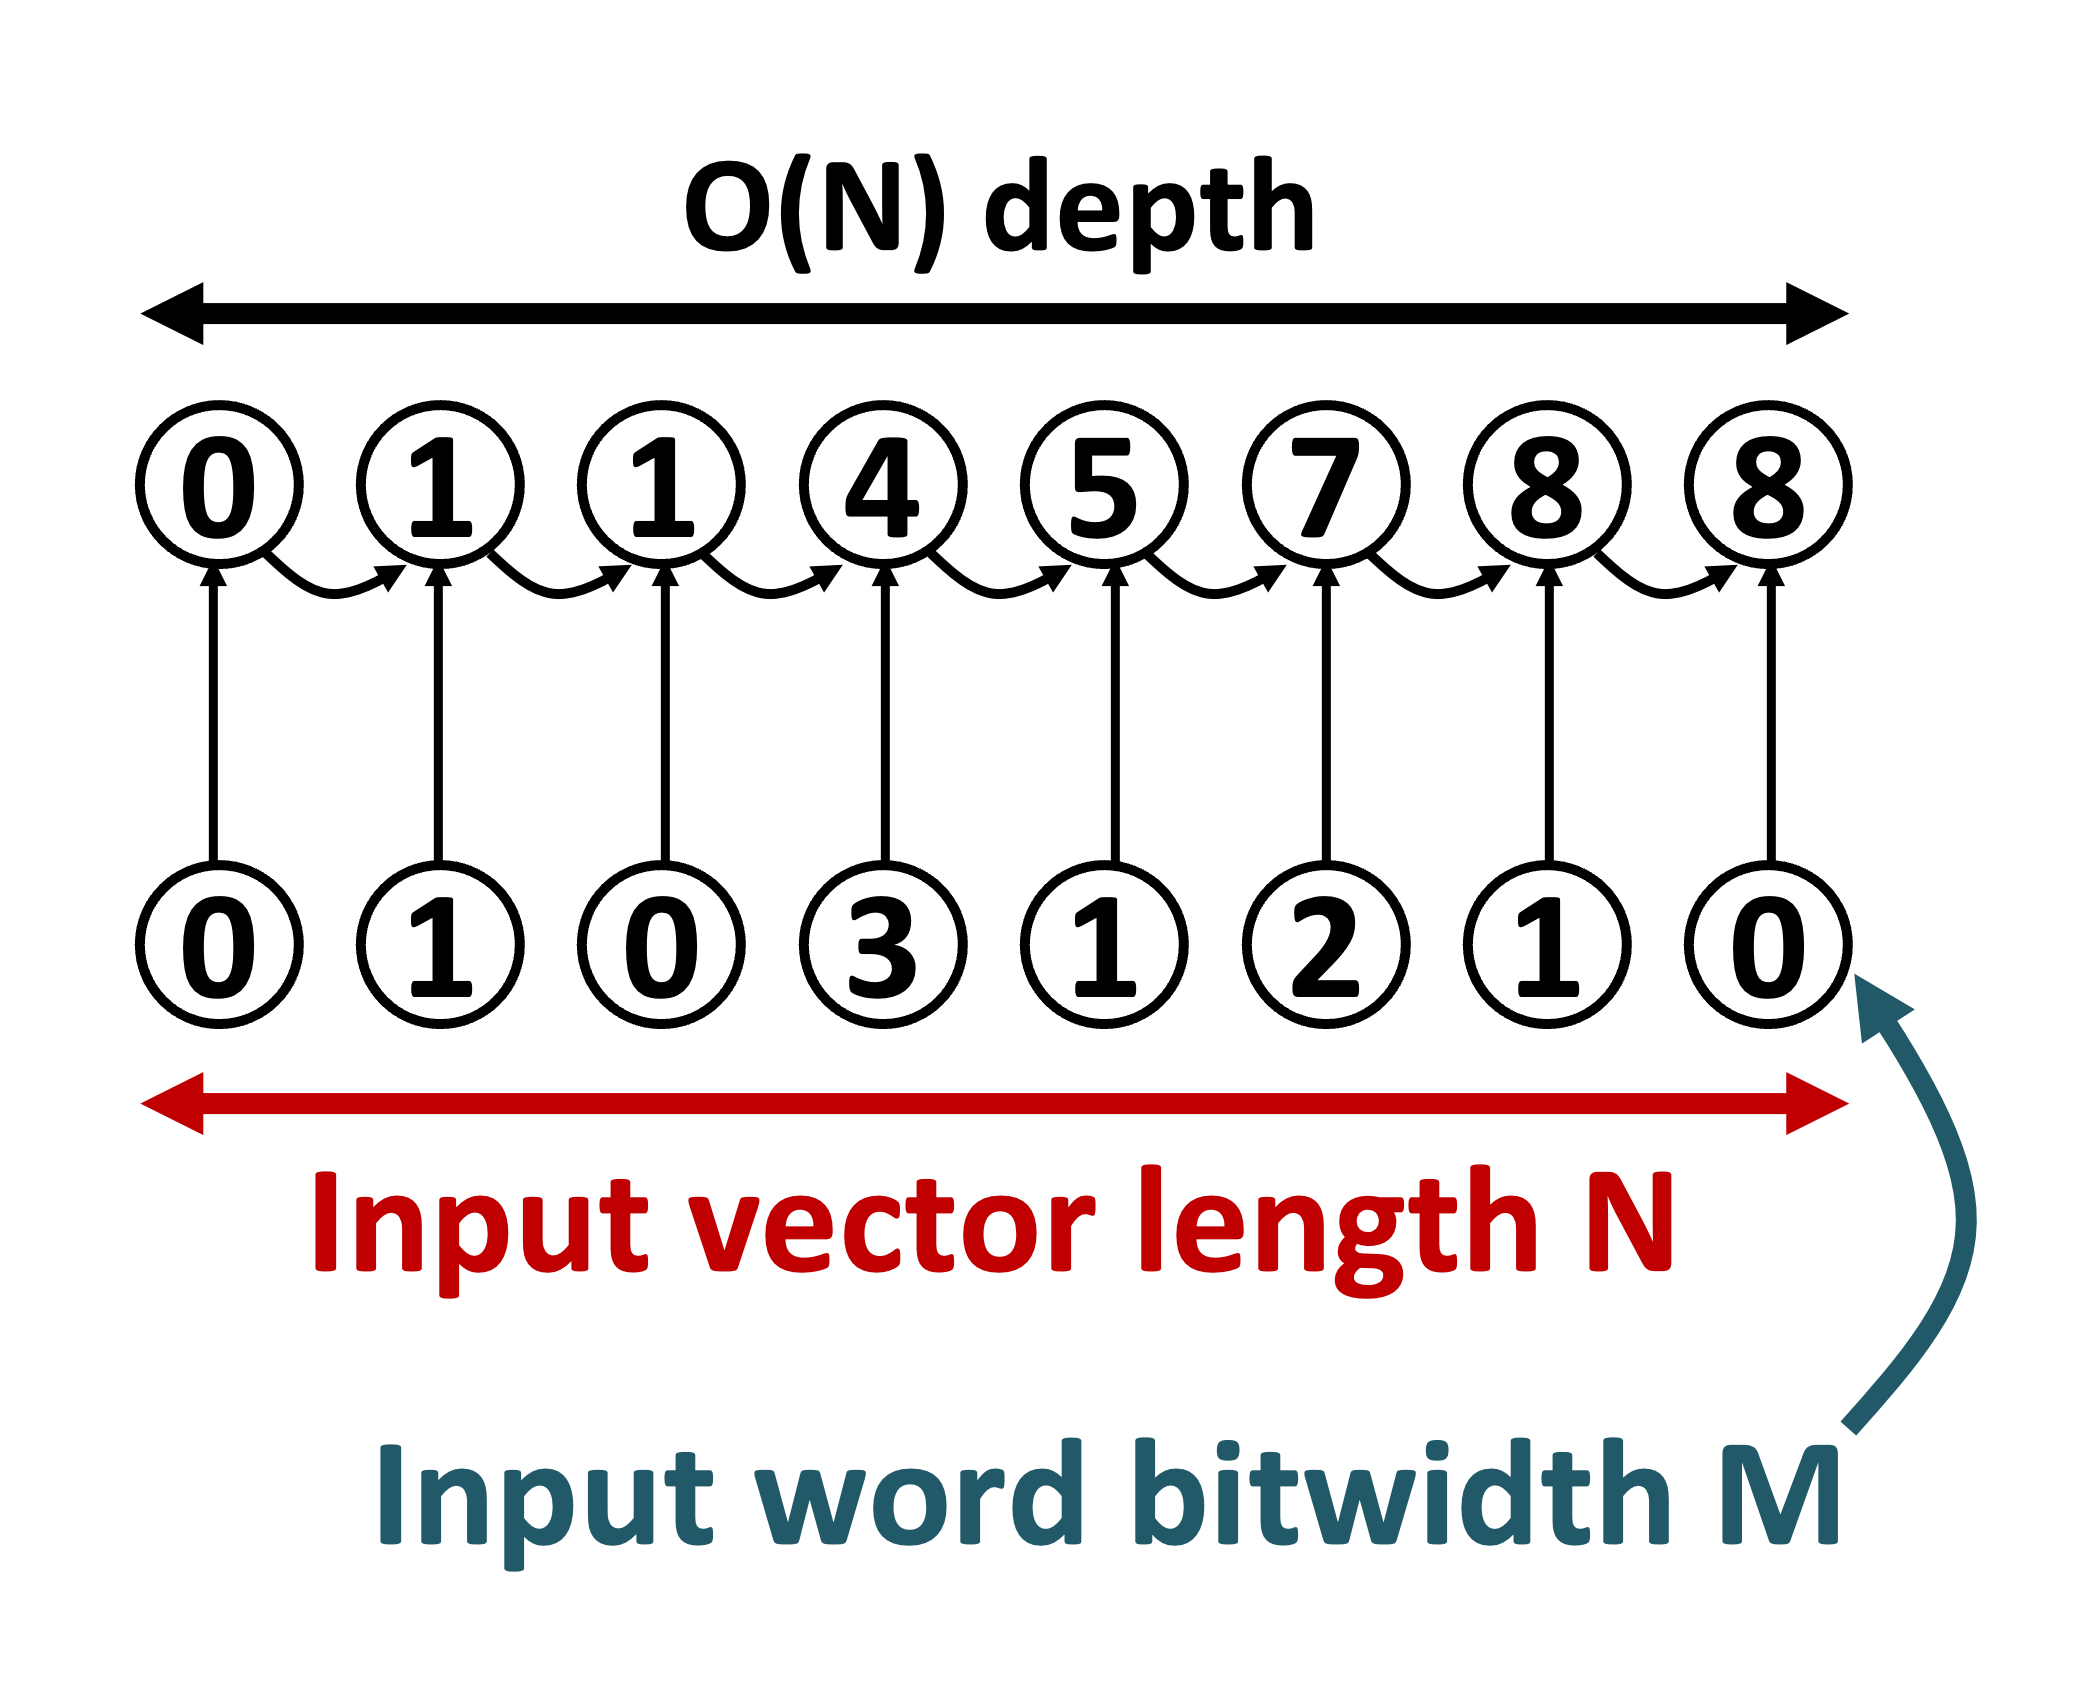
\includegraphics[width=0.95\textwidth]{figures/ripple_prefix_sum.png}
    \caption{The ripple prefix-sum RTL block implements a linear-depth vectorized prefix-sum. It is parameterized by \textbf{input word bitwidth} and \textbf{degree of vectorization.} This RTL block is implemented as a 1-stage vector pipeline (registered I/O) however the combinational design is not ``parallel'' and propagation delay is linear in the degree of vectorization.}
    \label{fig:ripple_prefix_sum}
\end{figure}

Figure~\ref{fig:ripple_prefix_sum} summarizes ripple prefix-sum.

\subsection{Priority encoder units}

Priority encoder requires either vector pipelining or combinational unrolling in order to support output throughput greater than 1.

\textbf{Vector priority encoder parameters:}

\begin{itemize}
    \item Number of input bits
    \item Output vector size
    
    \begin{itemize}
        \item Meaning: if the output vector size is $k$, a vectorized priority encoder returns a vector of indices for the top-$k$ priority hot bits in the input vector. 
        \item If the input bitmask contains $n < k$ hot bits, the priority encoder returns a length-$k$ vector with the $n$ hot-bit indices compacted into the first $n$ vector elements; vector elements at offsets $>n-1$ are undefined.
    \end{itemize}

\end{itemize}

\textbf{RTL implementations for the following priority encoder designs (all sharing the above parameter list) are provided:}

\begin{itemize}
    \item \textbf{Parallel decimation-by-2 priority encoder\cite{recursive_priority_encoder}:} log-depth, decimation-by-2 parallel priority encoder design.
\end{itemize}

\subsection{Intersection units}

Several intersection unit varieties are explored in this work:

\begin{itemize}
    \item ExTensor-like\cite{extensor} naive two-finger intersection
    \item ExTensor-like\cite{extensor} optimized intersection unit
    \item SparTen-like\cite{sparten} Bitmask intersection unit
    \item Direct-mapped intersection unit, a potentially novel intersection unit design developed for this work.
\end{itemize}

Both ExTensor-like intersection units require either vector pipelining or combinational unrolling in order to support output throughput greater than 1.

\subsubsection{Two-finger intersection unit (``ExTensor-naive-like'')}

% Radix-2 intersection overview figure
\begin{figure}[H]
    \centering
    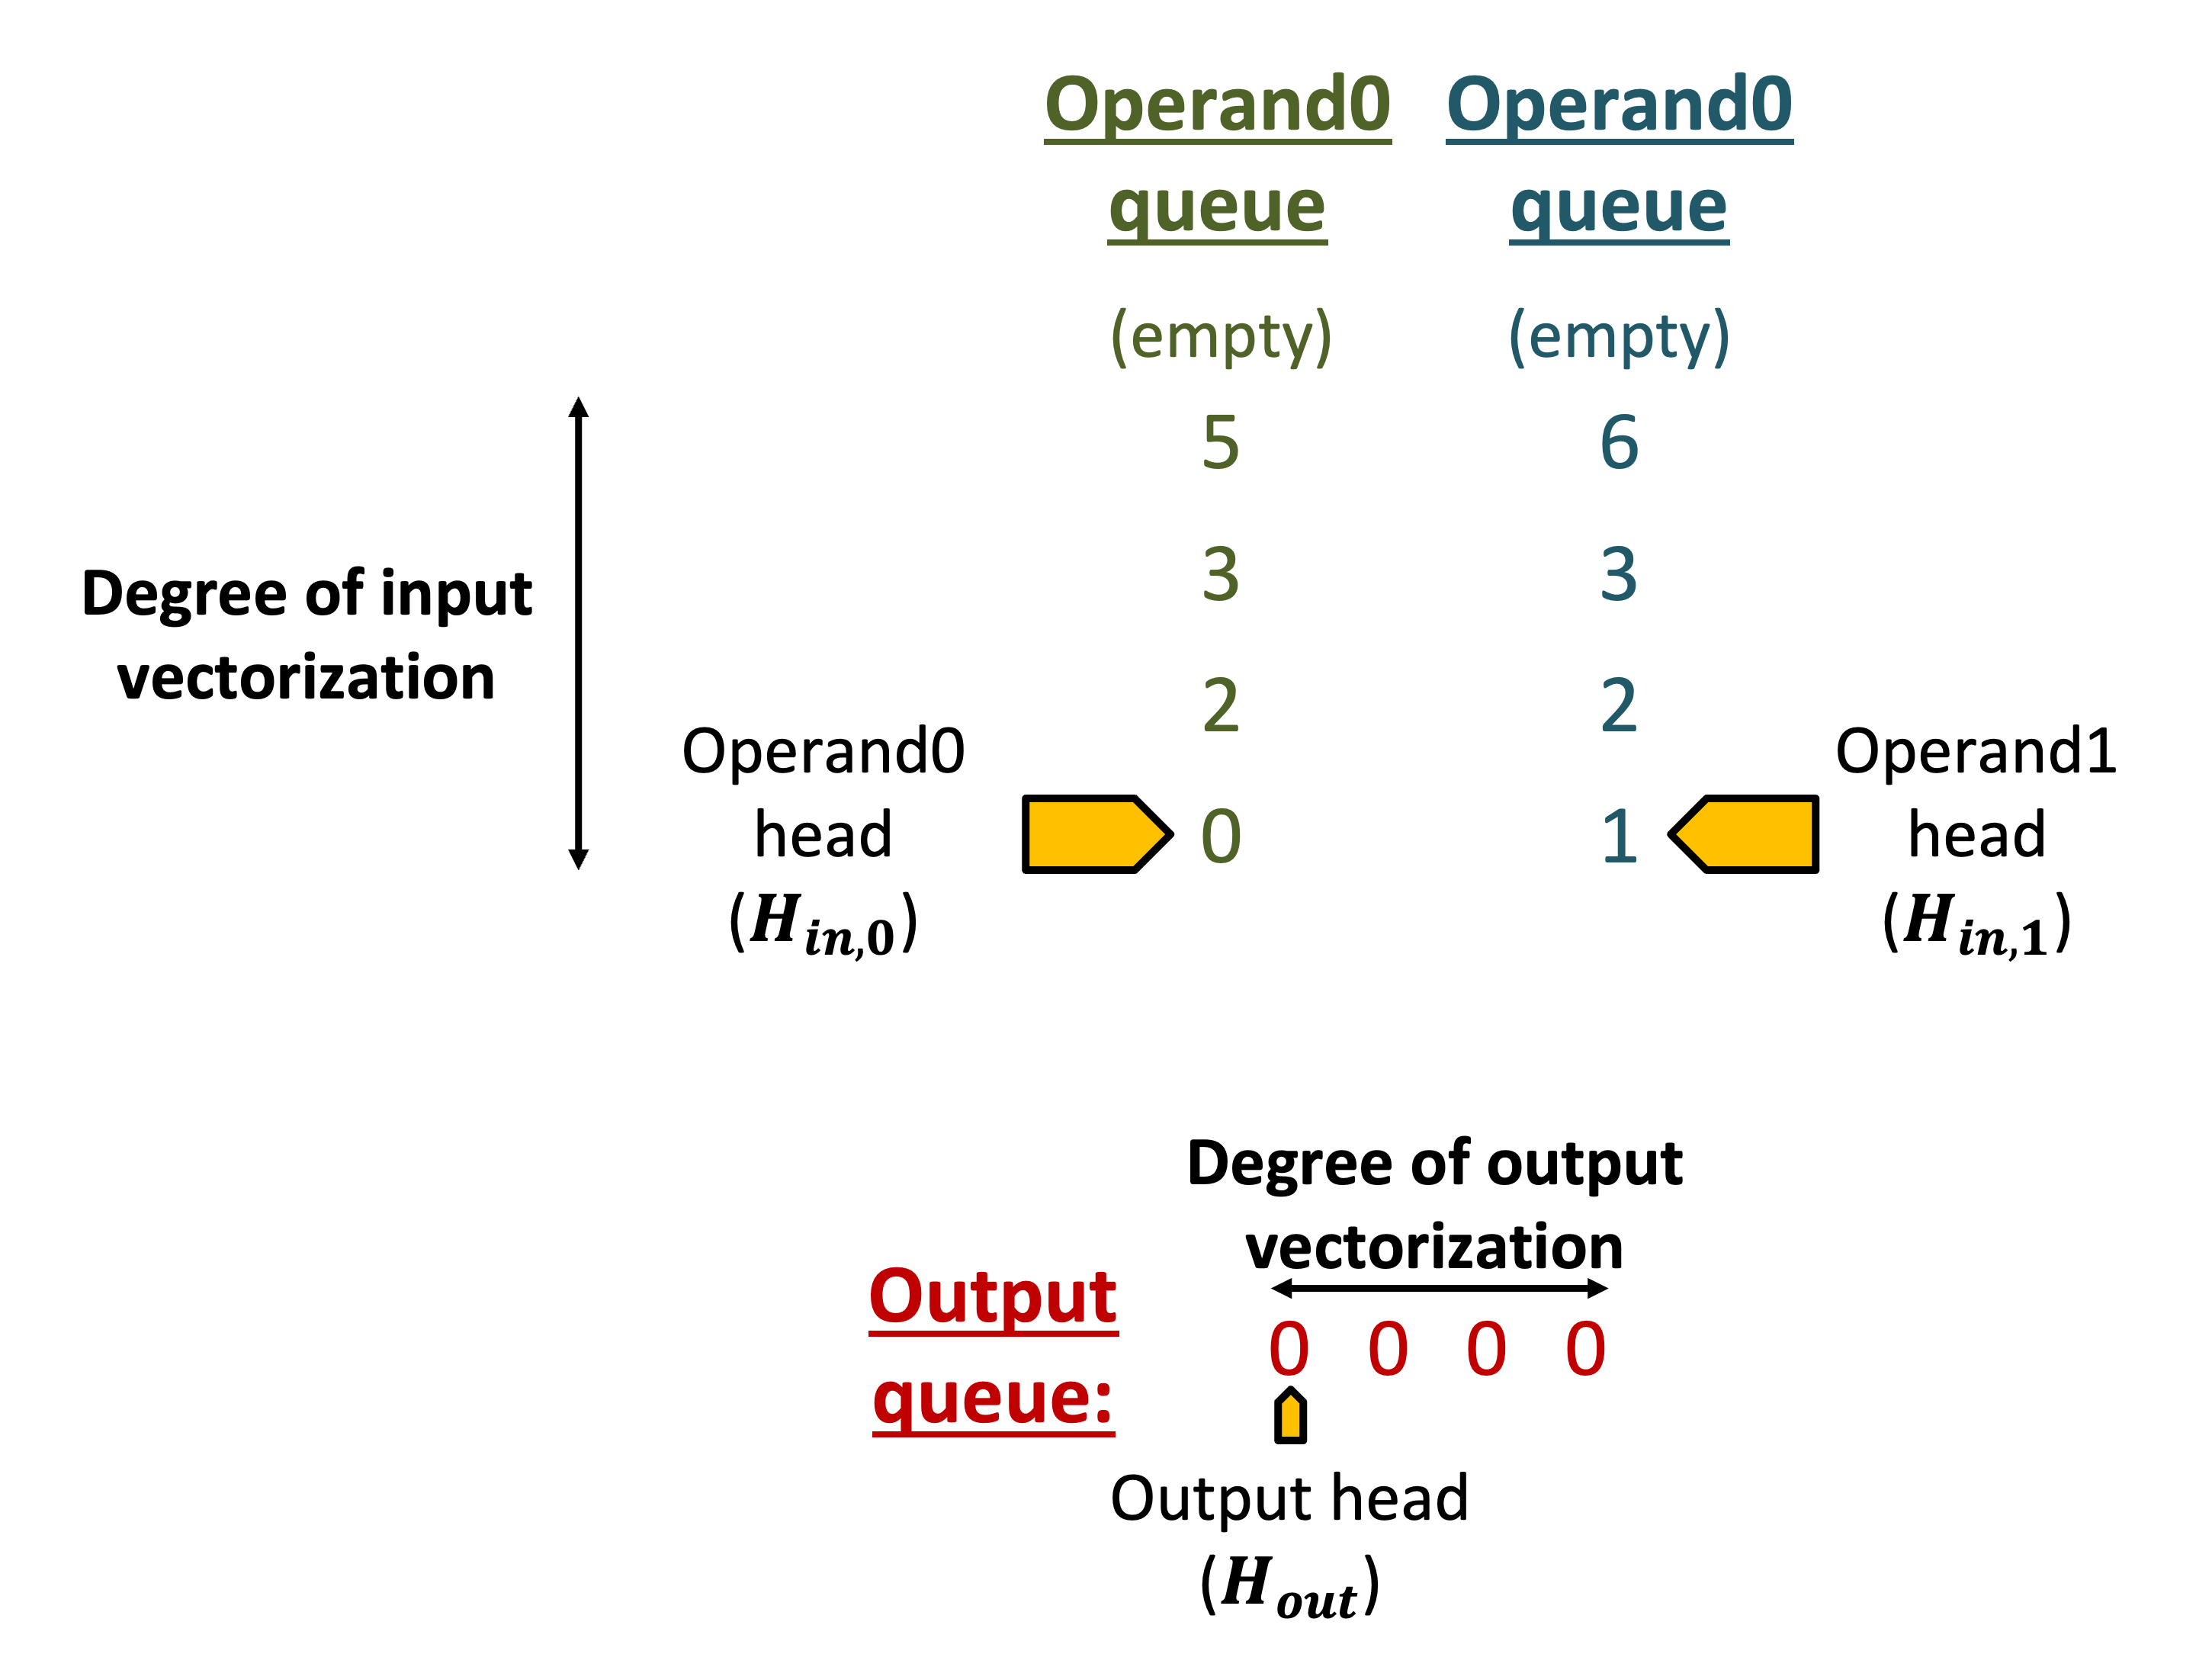
\includegraphics[width=\linewidth]{figures/radix2_intersect_overview.png}
    \caption{Overview of two-fingered intersection unit}
    \label{fig:radix2-overview}
\end{figure}

% Radix-2 intersection example figure
\begin{figure}[H]
    \centering
    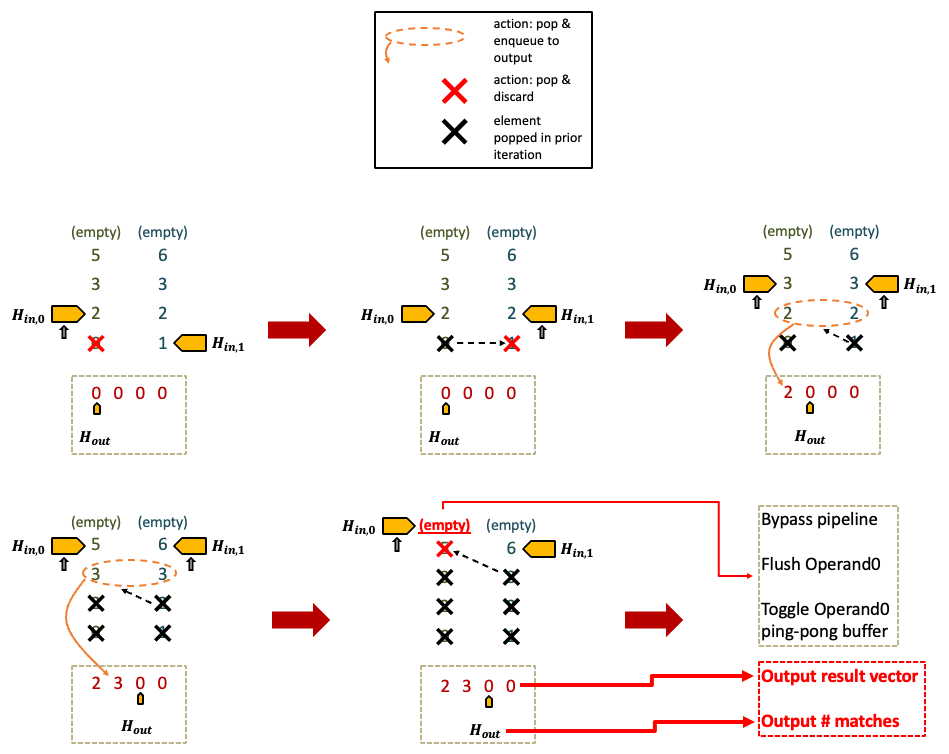
\includegraphics[width=\linewidth]{figures/radix2_intersect_example.png}
    \caption{Example of Radix2 Intersection}
    \label{fig:radix2-example}
\end{figure}

The two-finger intersection unit, modeled off of ExTensor\cite{extensor}, is similar to a radix-2 merge except it only outputs a value when the heads of the two lists are equal. This is exemplified in Figure~\ref{fig:radix2-overview} and Figure~\ref{fig:radix2-example}. Figure~\ref{fig:radix2-example} shows how the lowest element is popped for either vector, iteratively, until one or both vectors are empty. If the heads of the vectors are equal, both vectors are popped and the matching value is integrated into the output vector.

% Radix-2 intersection overview figure
\begin{figure}[H]
    \centering
    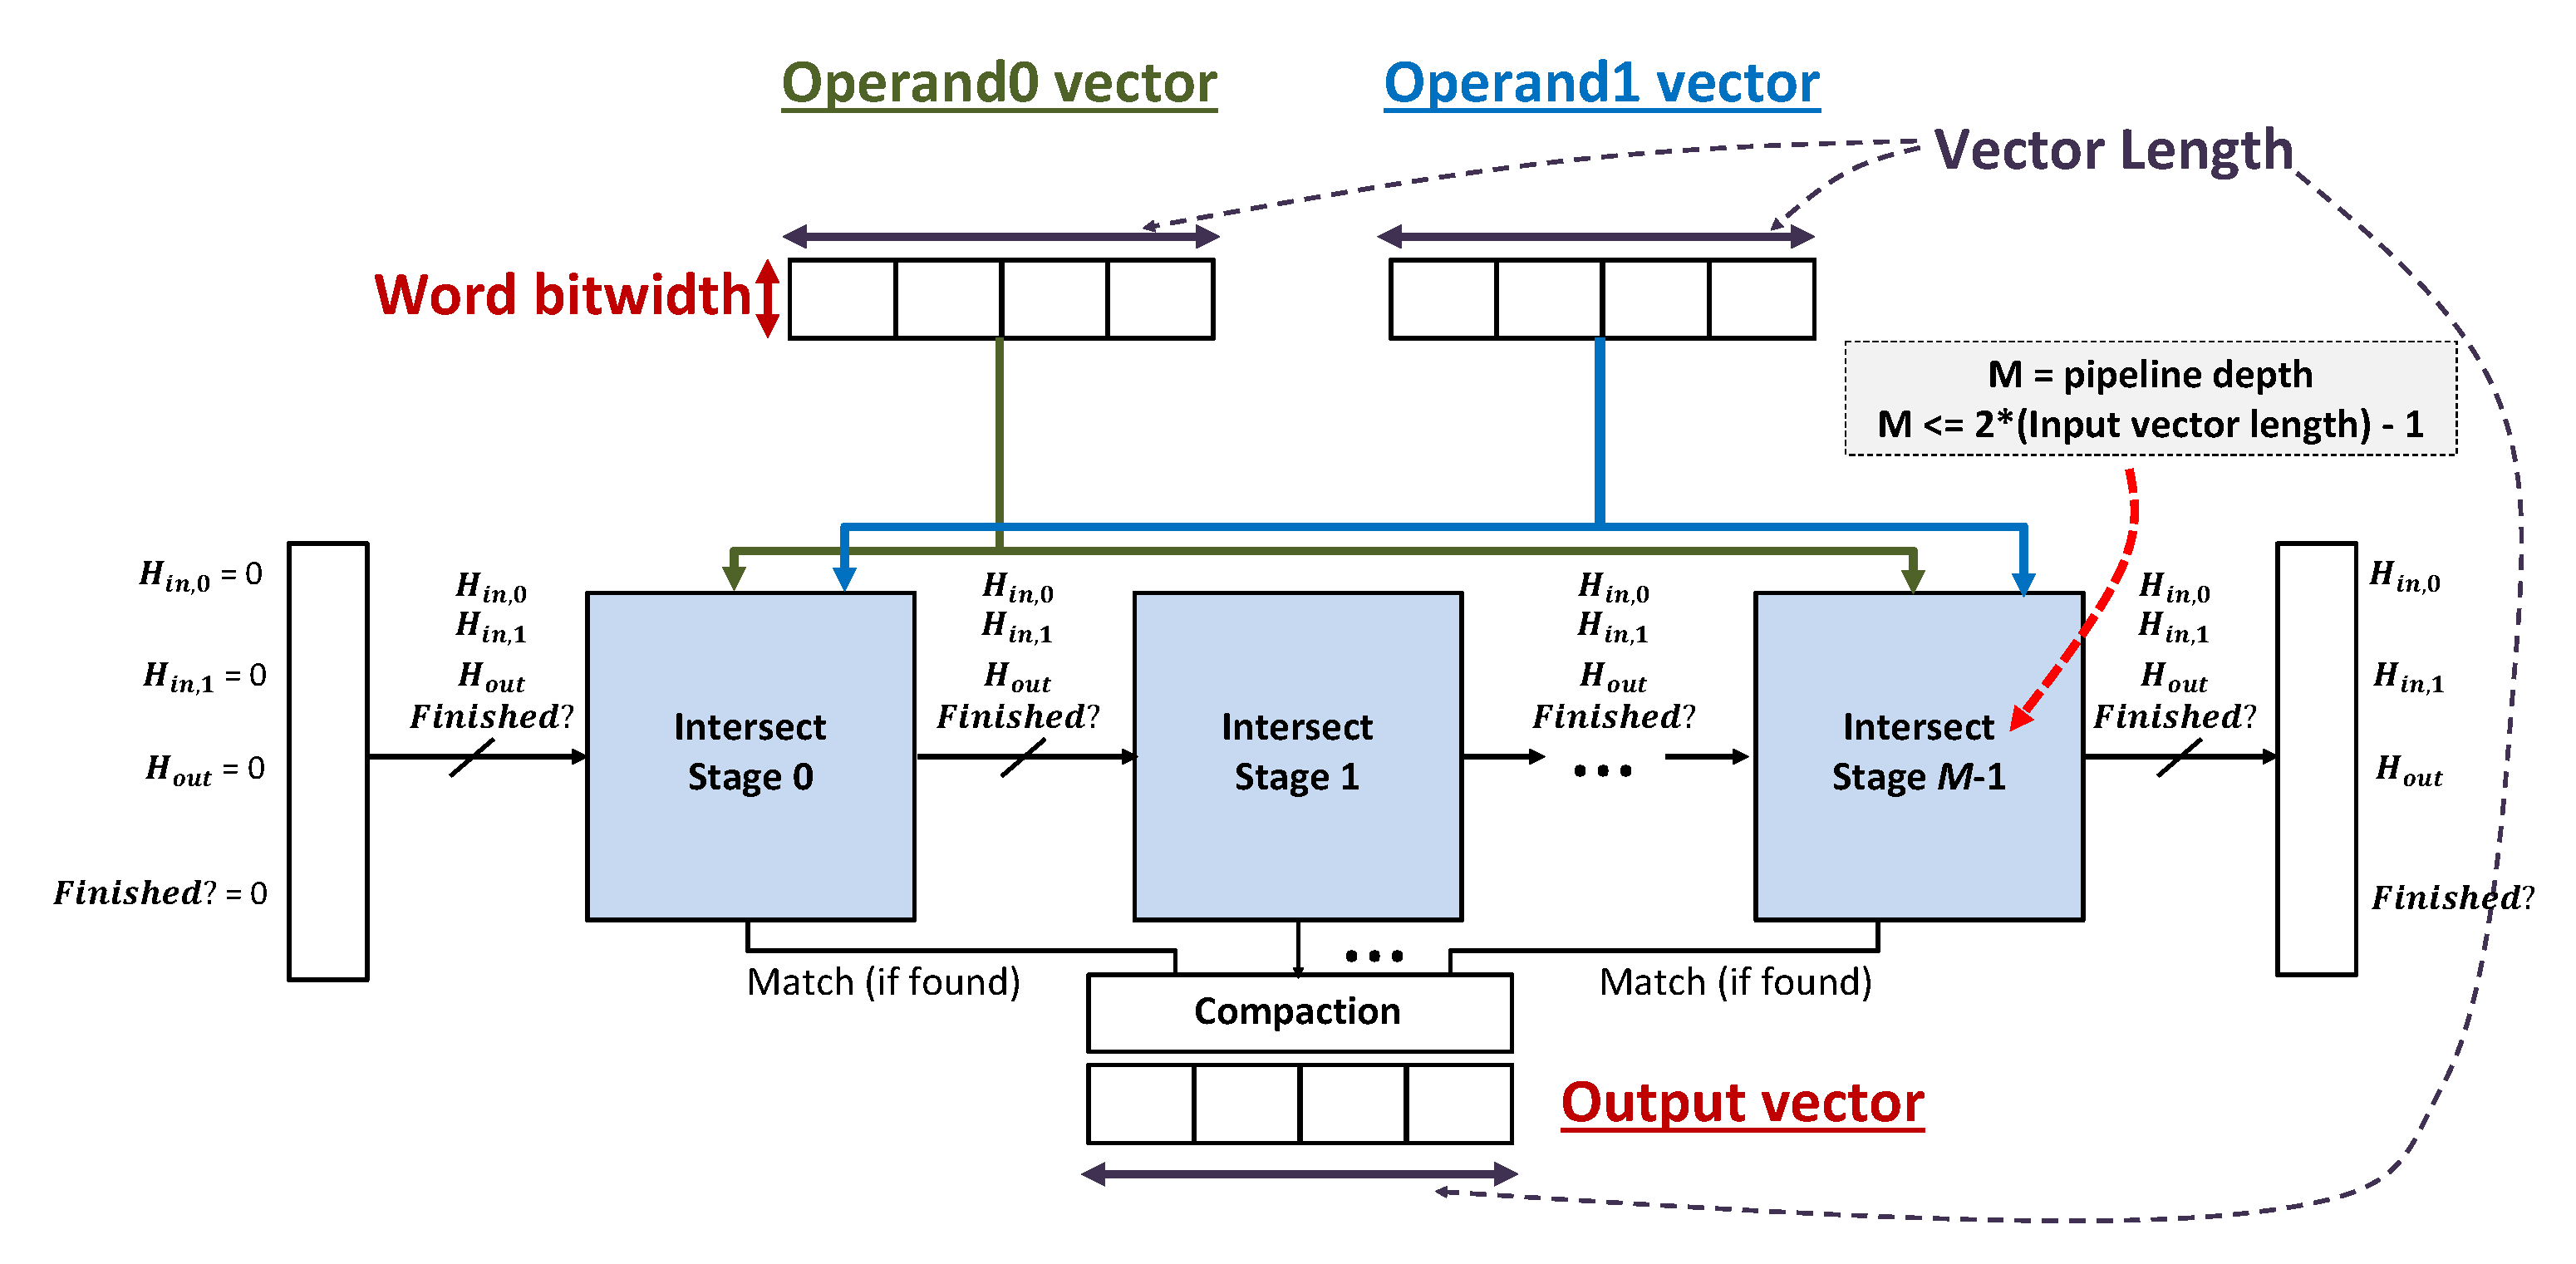
\includegraphics[width=\linewidth]{figures/two_finger_merge_pipeline.pdf}
    \caption{Two-fingered intersection vector pipelining or combinational unrolling.}
    \label{fig:radix_2_vector pipeline}
\end{figure}

Figure~\ref{fig:radix_2_vector pipeline} shows the approach to implementing vector pipelining or combinational unrolling for the two-fingered intersection unit. A stage vector enters the pipeline on the left, and an updated state vector exits on the right. The two operand vectors enter from above and are shared between each stage; in combinational unrolling, the need for multiple read/write ports can potentially lead to non-linear overheads. Special compaction logic compacts all matches from all stages into an output vector.

The state vector includes a ``Finished?'' signal, triggered when one or both lists are empty; when a stage raises this signal, all subsequent stages are bypassed.

\subsubsection{``Skip-ahead'' intersection unit (``ExTensor-optimized-like'')}

The skip-ahead intersection unit - also inspired by ExTensor\cite{extensor} - uses an optimized content-aware search process to increase the probability of finding an intersection match.

\begin{figure}[ht]
\centering
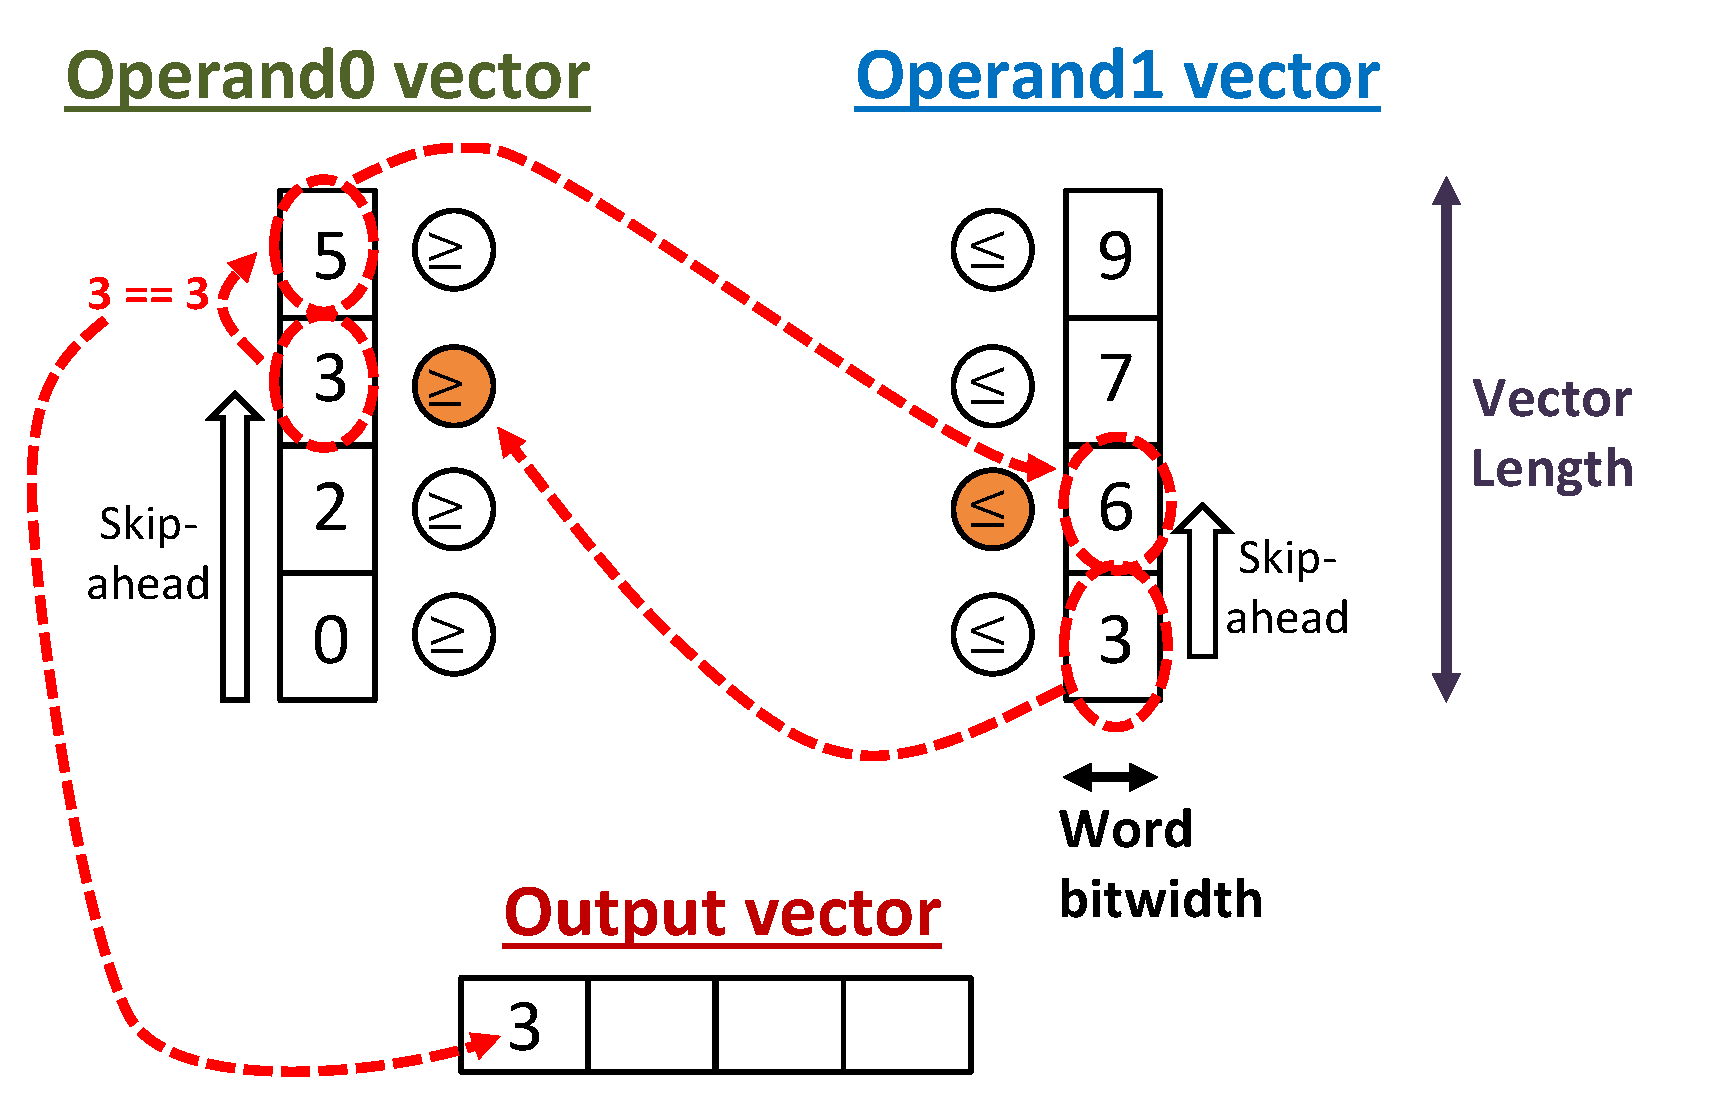
\includegraphics[width=0.7\textwidth]{figures/skip_ahead_dia.pdf}
\caption{.}
\label{fig:skip_ahead_dia}
\end{figure}

Figure~\ref{fig:skip_ahead_dia} illustrates how the content-aware search allows the intersection unit to ``skip-ahead'': by using content-addressable memories (CAMs), the control logic associated with the Operand1 vector can find the first element of Operand0 which is equal or greater than the head of Operand1, in a single step. 

Otherwise, the implementation of combinational unrolling/vector pipelining for skip-ahead intersection is identical to Figure~\ref{fig:radix_2_vector pipeline}.

\subsubsection{Parallel direct-mapped intersection unit}

The parallel direct-mapped intersection unit is a potentially novel intersection unit design developed for this work.

It finds all matches between two vectors in a single cycle, without pipelining or combinational unrolling.

This design intersects two vectors of sorted coordinate metadata, and outputs a third sorted vector of common metadata values between the two input vectors. 

\clearpage

\begin{figure}[H]
    \centering
    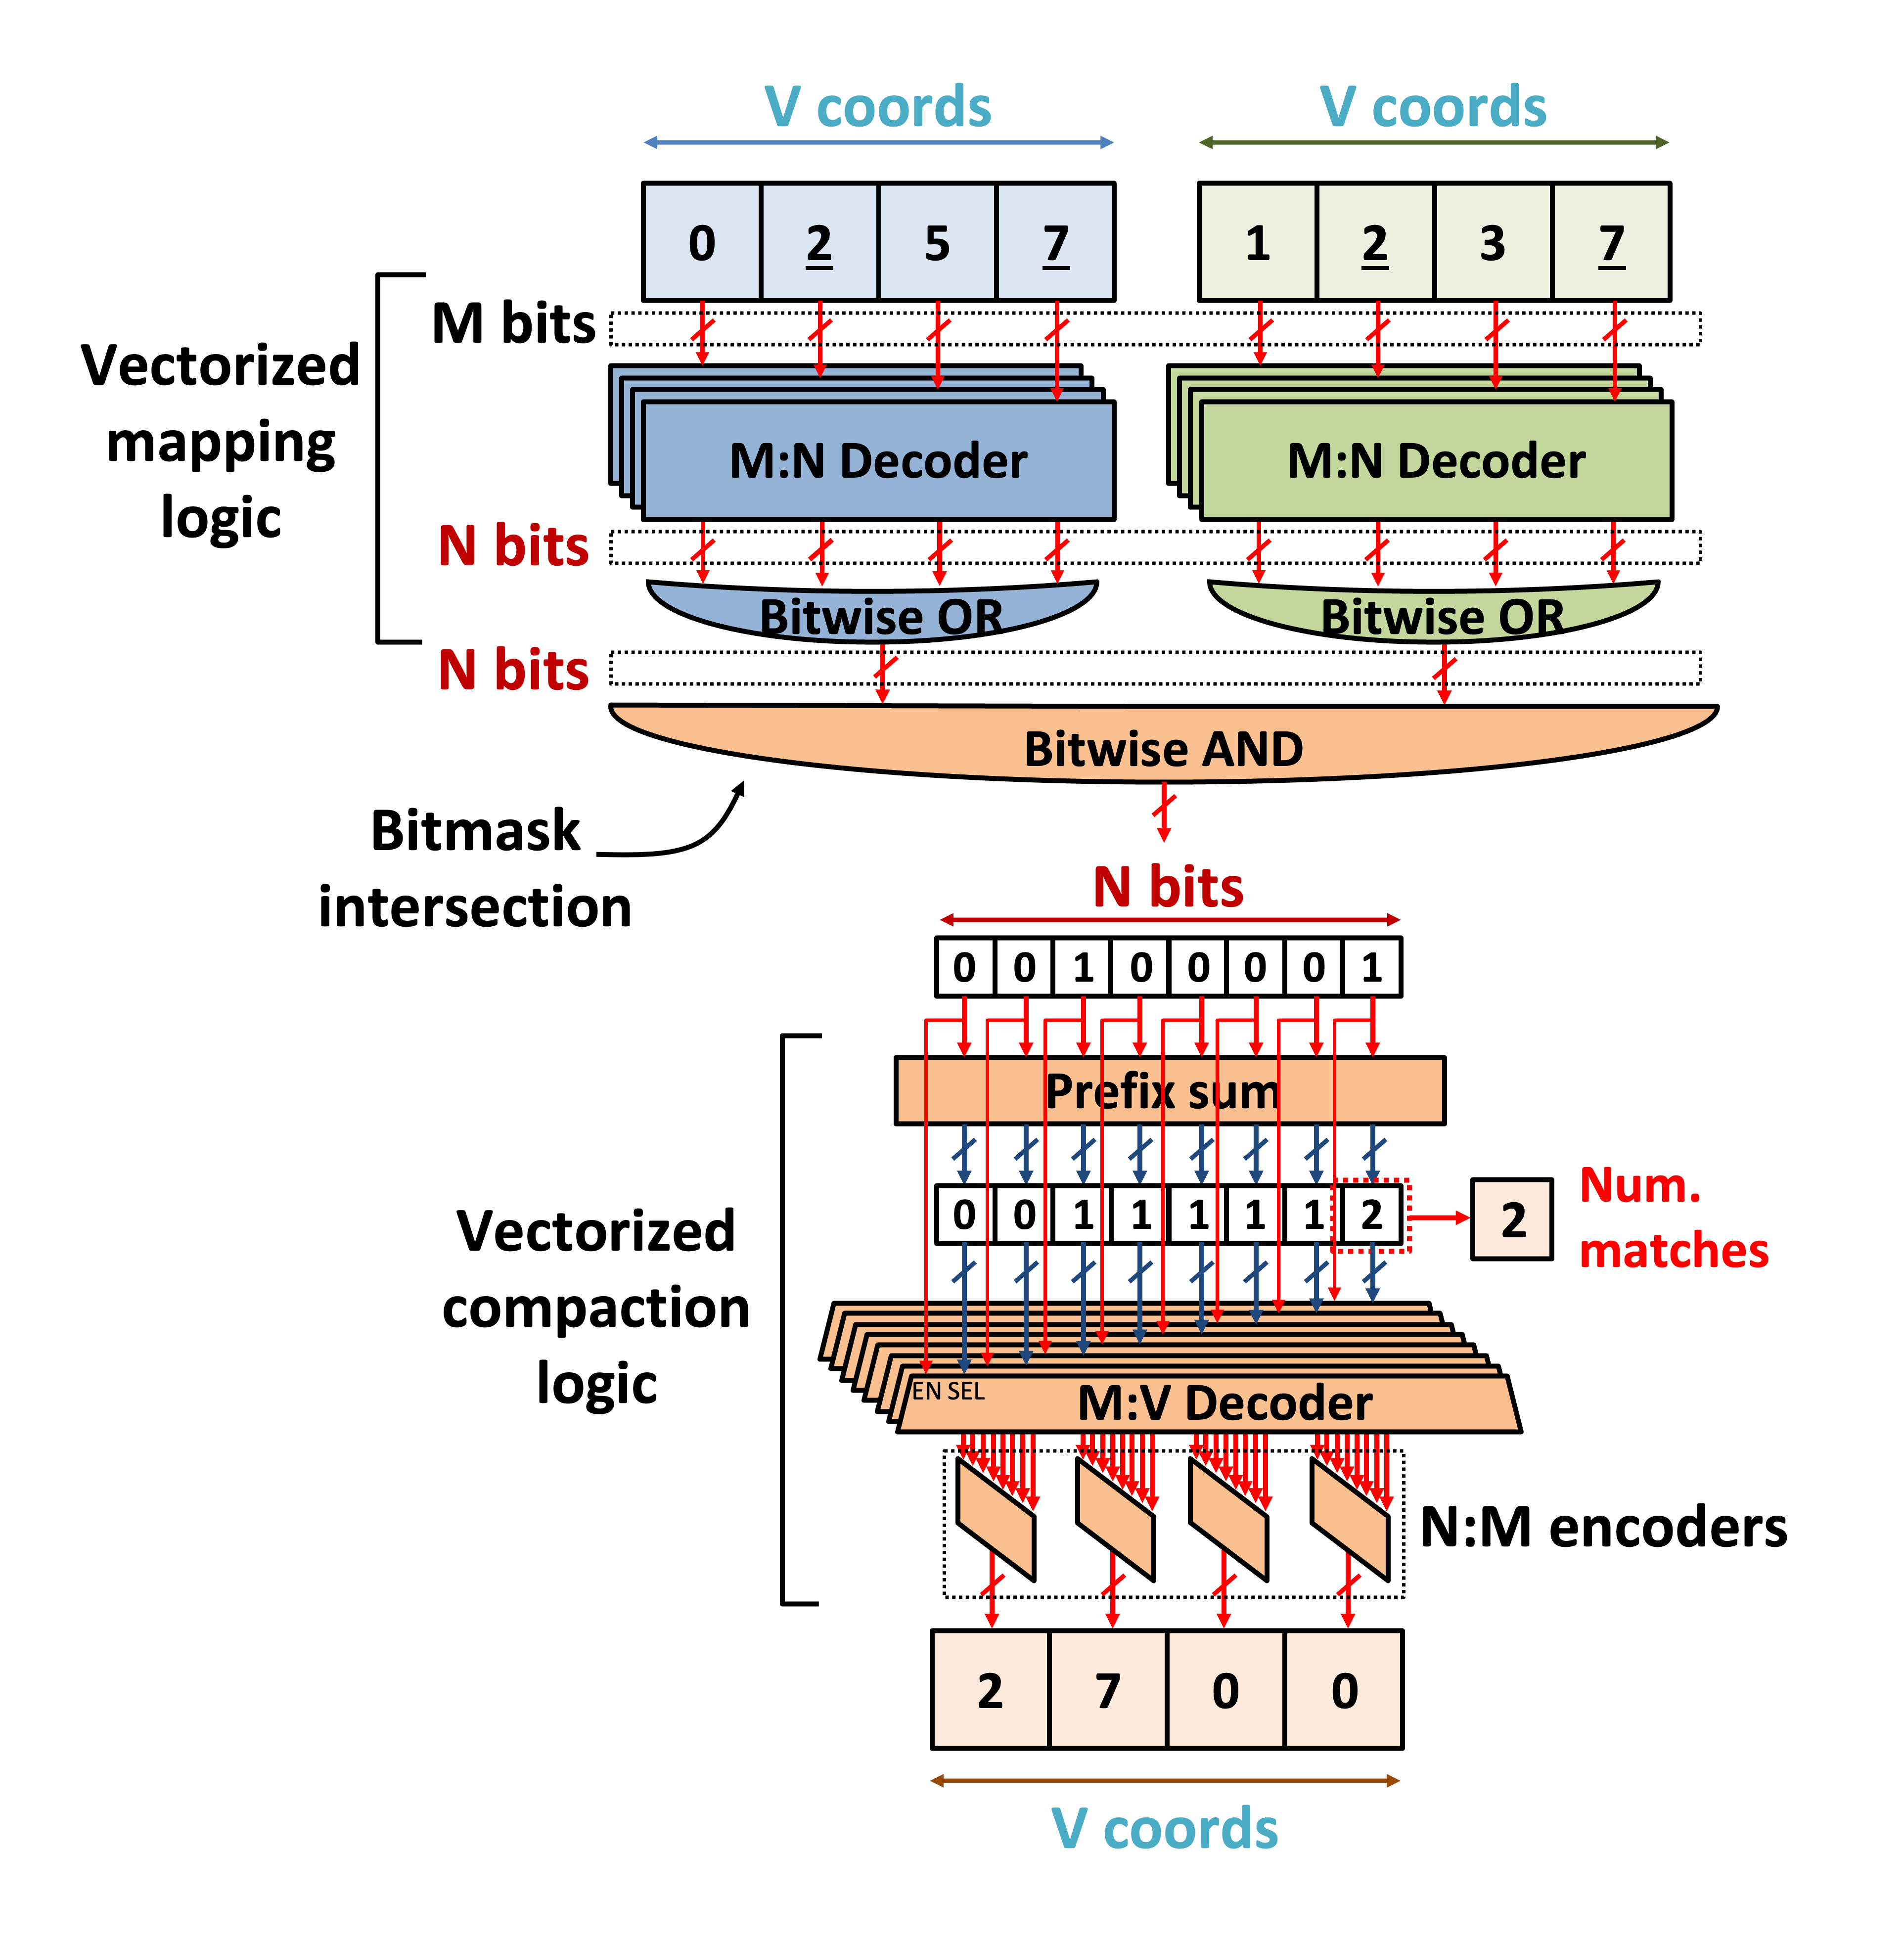
\includegraphics[width=0.95\textwidth]{figures/direct_mapped_isect.png}
    \caption{Vectorized direct-mapped intersection unit. Consumes two coordinate metadata vectors, and outputs a compacted and sorted vector of common elements, along with a count of common elements ($num\_matches$.) Output vector indices greater than $num\_matches - 1$ have undefined values.}
    \label{fig:direct_mapped_isect}
\end{figure}

\clearpage

The implementation, shown in Figure~\ref{fig:direct_mapped_isect}, is based on a ``direct-mapped approach'', analogous to direct-mapped cache. An array of decoders maps the input vector operands from position-space into coordinate-space; this mapping is performed in parallel. This yields two bitmasks (one per operand); in a given operand's bitmask, the index of each hot bit corresponds to an explicit coordinate value in the corresponding input vector. A bitmask intersection is then performed, yielding a new bit-vector in which each hot bit corresponds to a \textit{common} explicit coordinate value between the two vectors. Compaction logic maps these common coordinates back into position-space, yielding a sorted vector of explicit coordinate values which are common to both input vectors.

\textbf{Vectorized parallel direct-mapped intersection unit parameters:}

\begin{itemize}
    \item Vector size (applies to input and output.)
    \item Fiber size (the coordinate-space length of the two sparse fibers being intersected.) This determines the size of the bitmasks.
    \item Coordinate metadata bitwidth, i.e. the number of bits per element in the input and output vectors.
\end{itemize}

For example, a fiber spanning the range of coordinate values $[0,L-1]$ would require the fiber size parameter to be set to L, regardless of the number of non-zero values in the fiber.



\subsubsection{Parallel bitmask intersection unit (SparTen\cite{sparten}-like)}

The parallel bitmask intersection unit is modeled after the bitmask intersection unit from SparTen\cite{sparten}. It operates exclusively on bitmask inputs, and finds all matches within a single cycle. It does not require vector pipelining or combinational unrolling.

\textbf{Vectorized parallel bitmask intersection unit parameters:}

\begin{itemize}
    \item Number of input bits
\end{itemize}

The parallel bitmask intersection unit applies a straightforward bitwise-AND operation and outputs the result.

% Bitmask intersection
\begin{figure}[H]
    \centering
    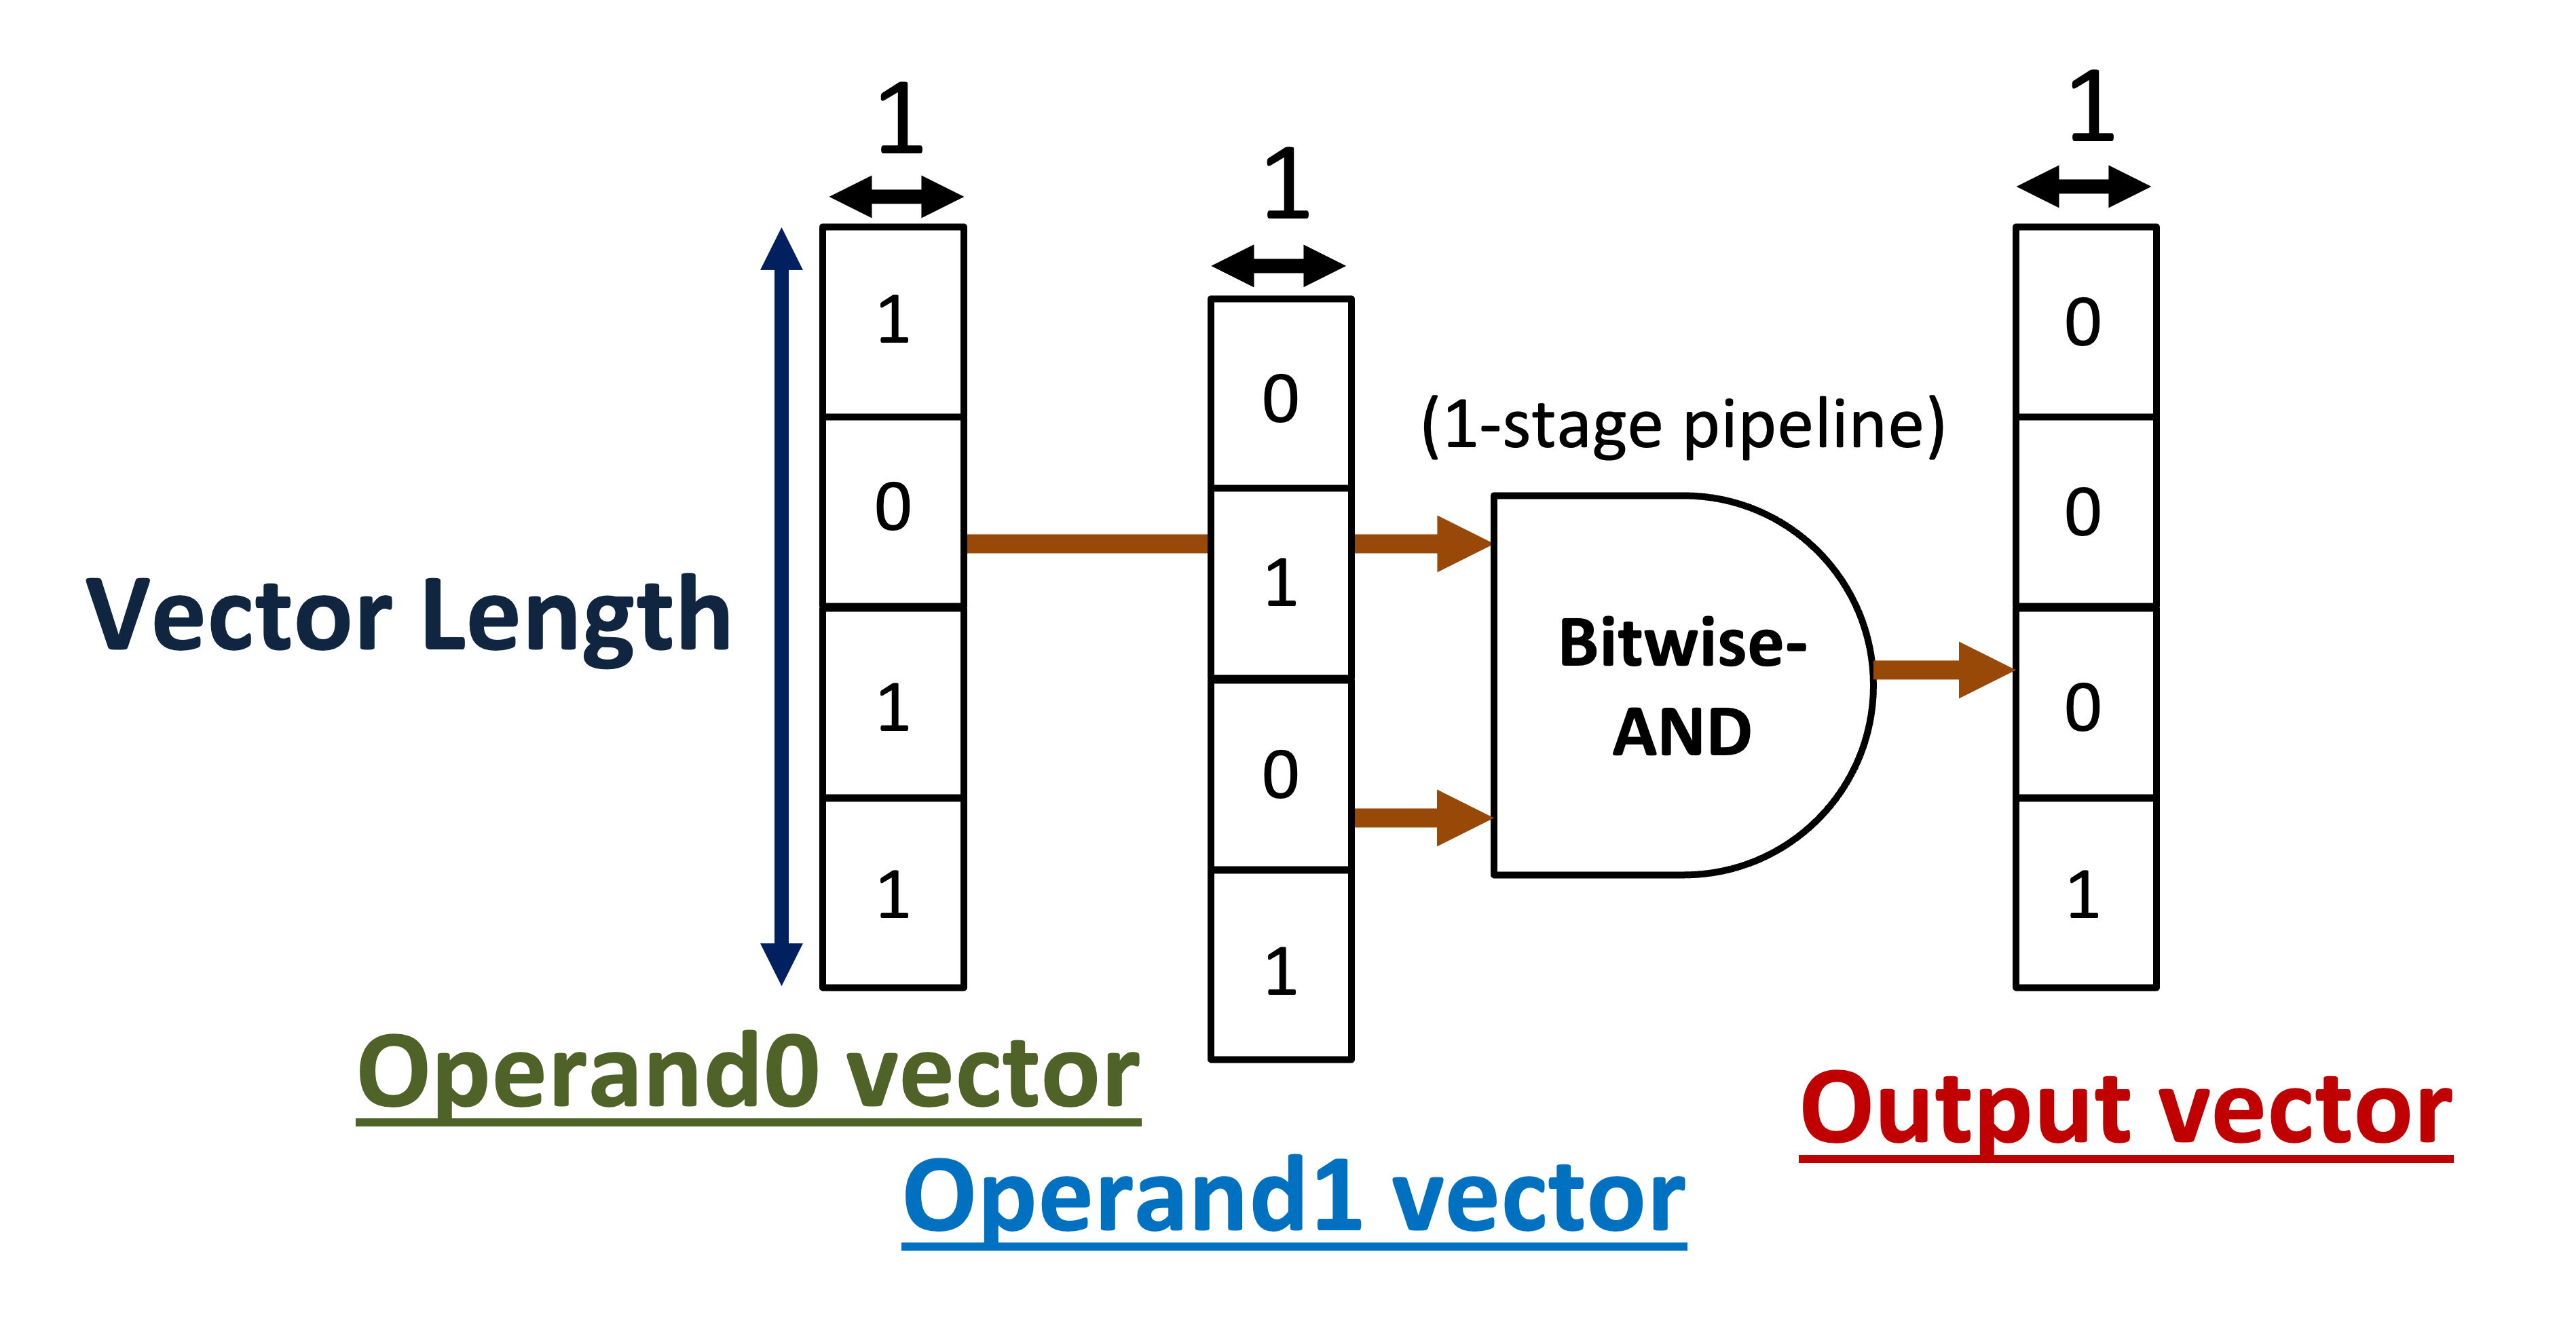
\includegraphics[width=\linewidth]{figures/bitmask_intersection.png}
    \caption{Bitmask intersection vector pipeline.}
    \label{fig:bitmask_intersection}
\end{figure}